\subsection{Komposisjon}

\begin{frame}{Relasjonskomposisjon}
    Gitt to relasjoner $R \subseteq A \times B$ og $S \subseteq B \times C$, kan vi konstruere komposisjonen $S \circ R \subseteq A \times C$:\\
    $S \circ R := \{(a, c) ~ | ~ (a, b) \in R, (b, c) \in S\}$
    \pause
    \begin{figure}%
        \centering
        \subfloat{{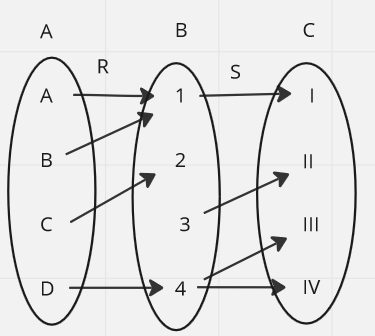
\includegraphics[width=3.3cm]{images/R, S.png} }}%
        \pause
        \qquad
        \subfloat{{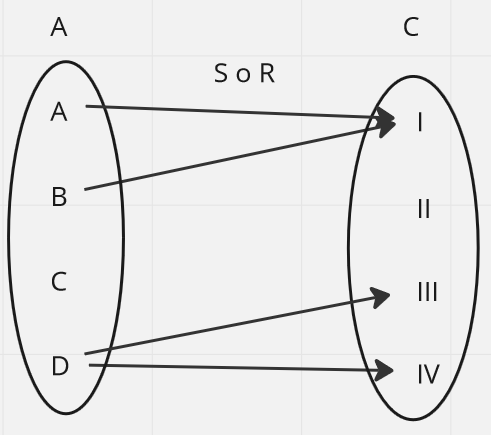
\includegraphics[width=3.3cm]{images/S o R.png} }}%
        \label{fig:ros}%
    \end{figure}
    \pause
    Obs! Som med funksjonskomposisjon er rekkefølgen er uintuitiv: R skjer før S.\\
    Dere kan lese det som $S$ 'på' $R$.
\end{frame}
